%\begin{figure*}[ht!]
%\centering
%\textbf{a) \textit{DaCapo}}\\
%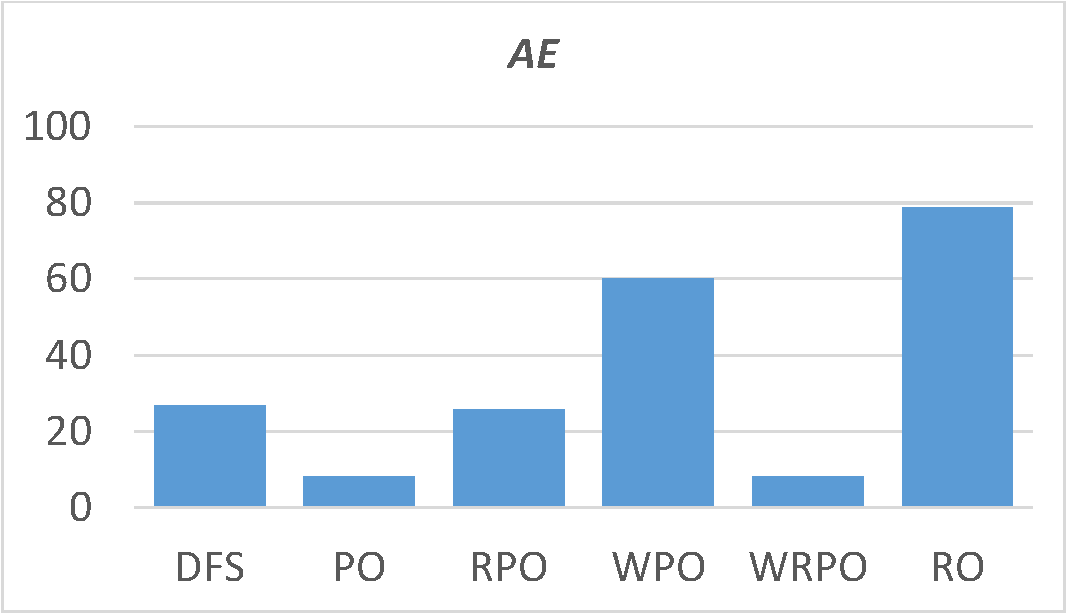
\includegraphics[width=0.32\linewidth]{ecoop-figures/ae-crop.pdf}
%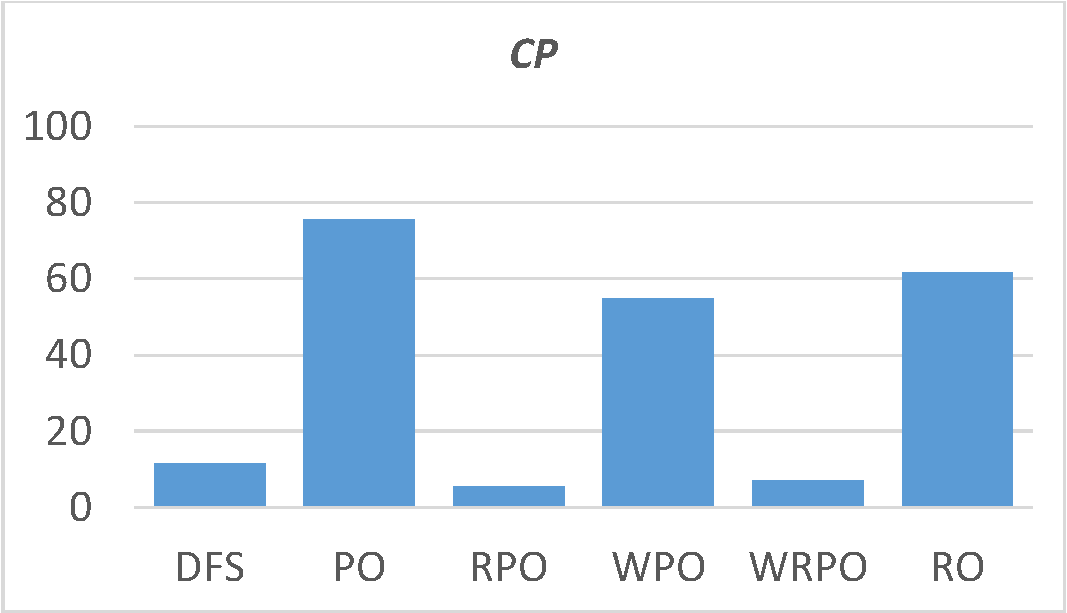
\includegraphics[width=0.32\linewidth]{ecoop-figures/cp-crop.pdf}
%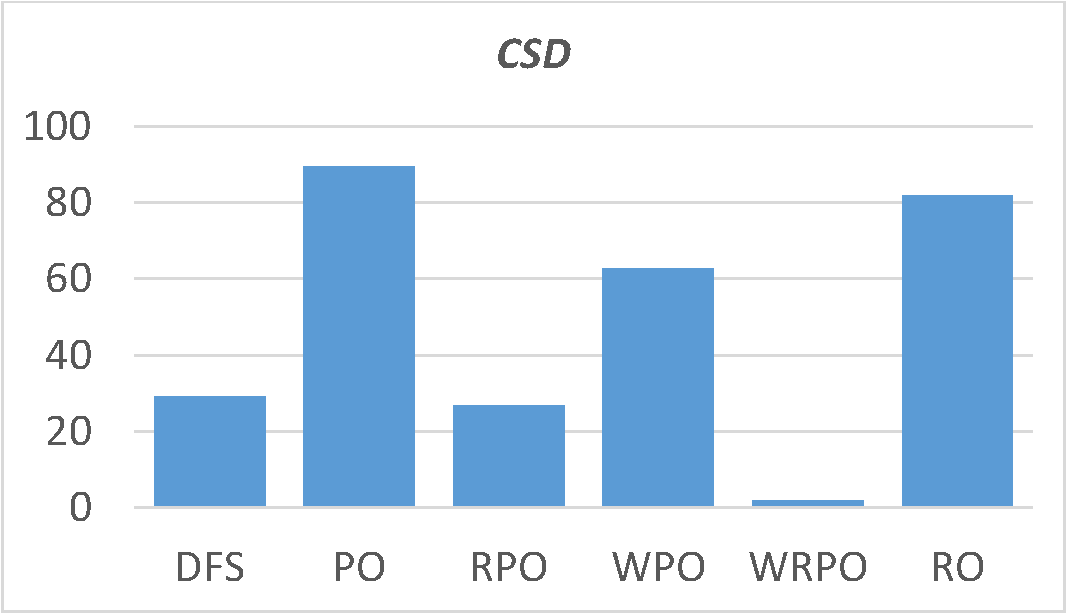
\includegraphics[width=0.32\linewidth]{ecoop-figures/csd-crop.pdf}
%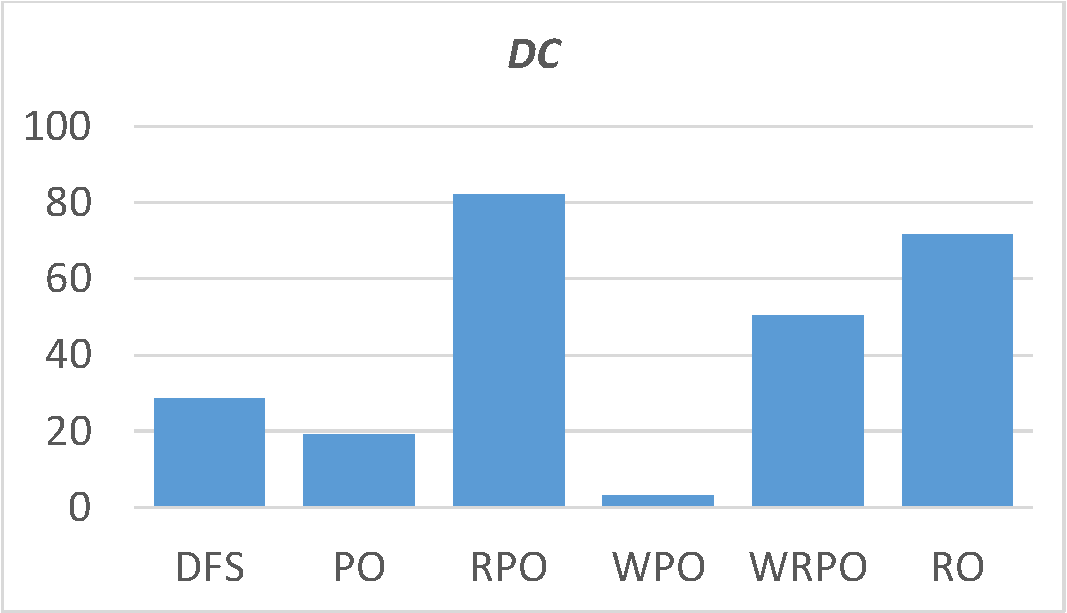
\includegraphics[width=0.32\linewidth]{ecoop-figures/dc-crop.pdf}
%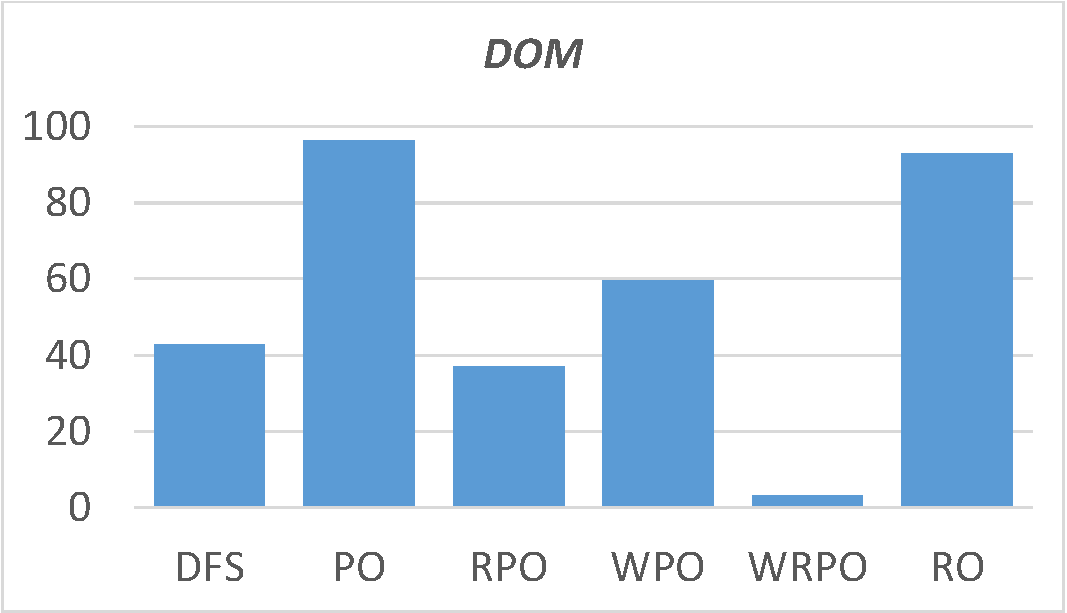
\includegraphics[width=0.32\linewidth]{ecoop-figures/dom-crop.pdf}
%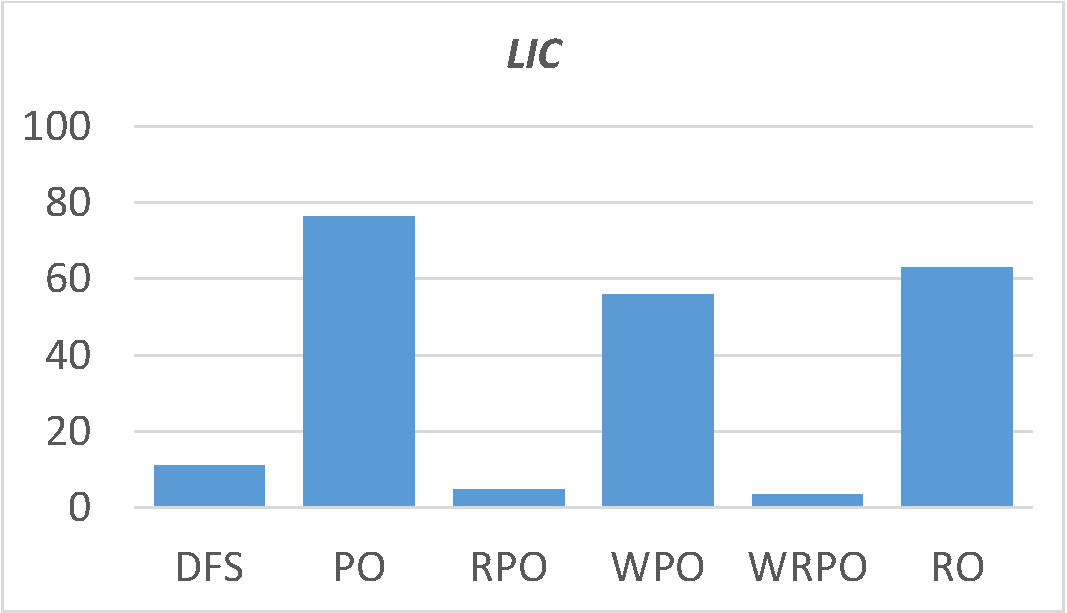
\includegraphics[width=0.32\linewidth]{ecoop-figures/lic-crop.pdf}
%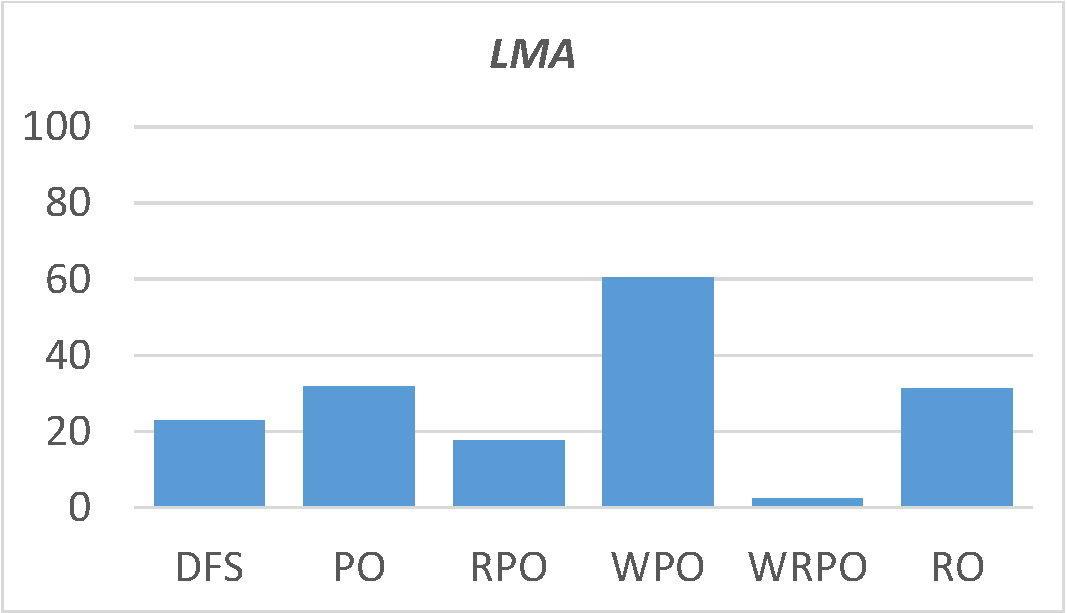
\includegraphics[width=0.32\linewidth]{ecoop-figures/lma-crop.pdf}
%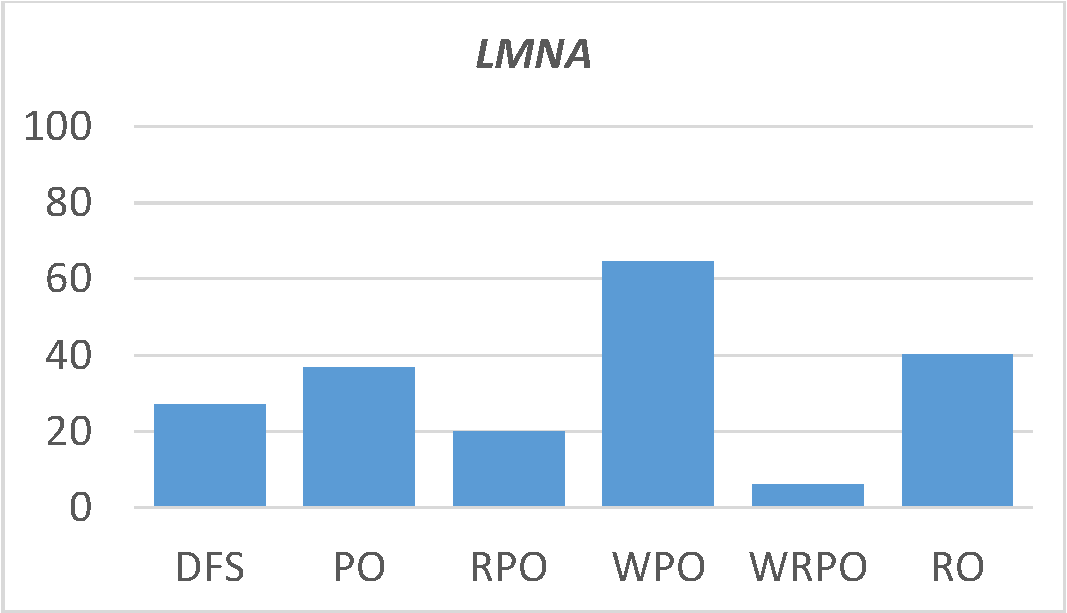
\includegraphics[width=0.32\linewidth]{ecoop-figures/lmna-crop.pdf}
%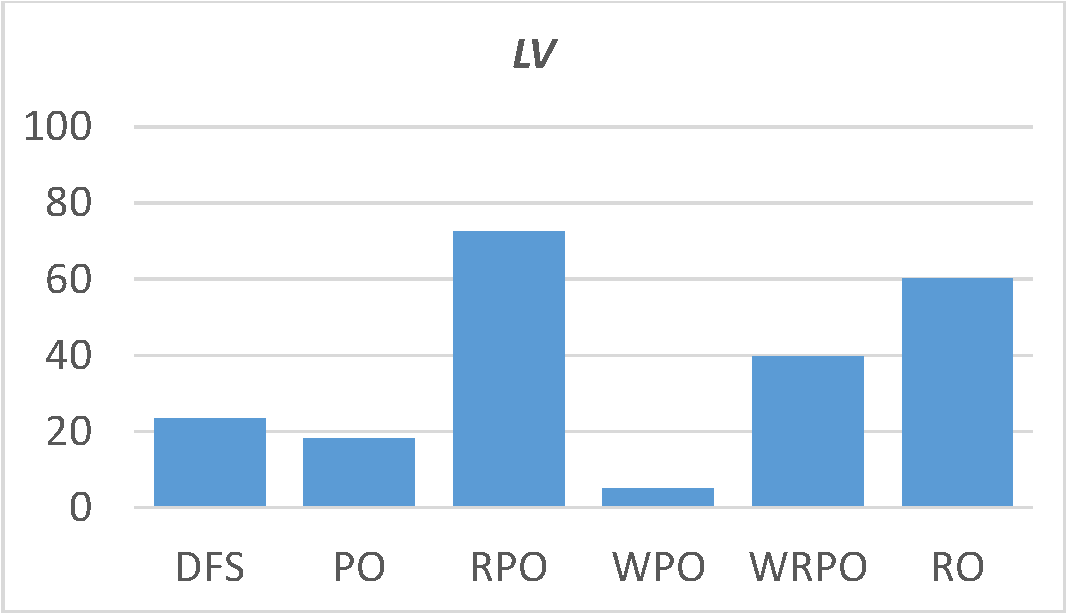
\includegraphics[width=0.32\linewidth]{ecoop-figures/lv-crop.pdf}
%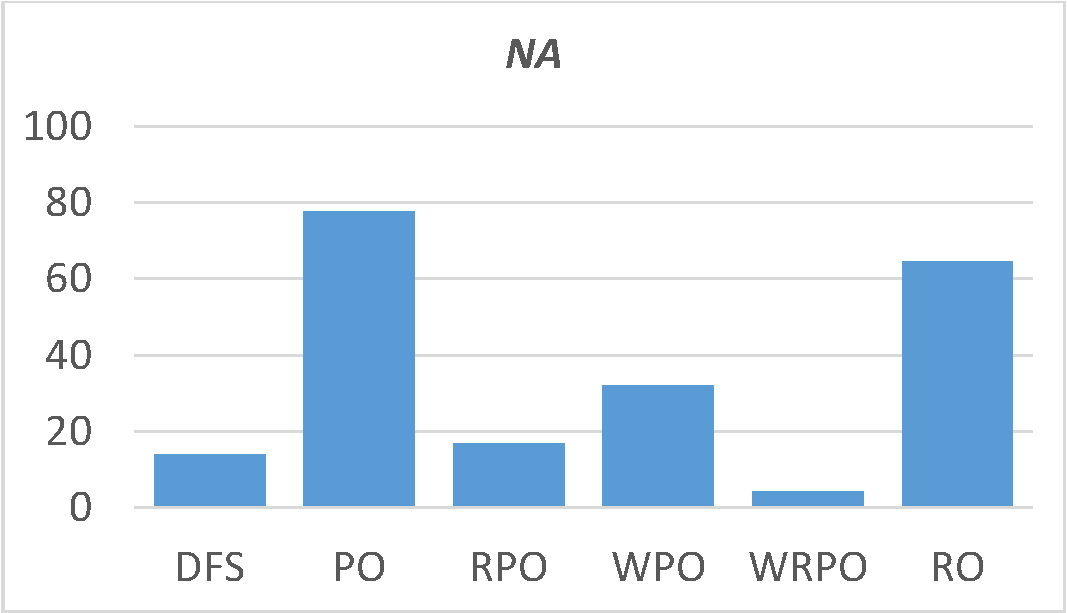
\includegraphics[width=0.32\linewidth]{ecoop-figures/na-crop.pdf}
%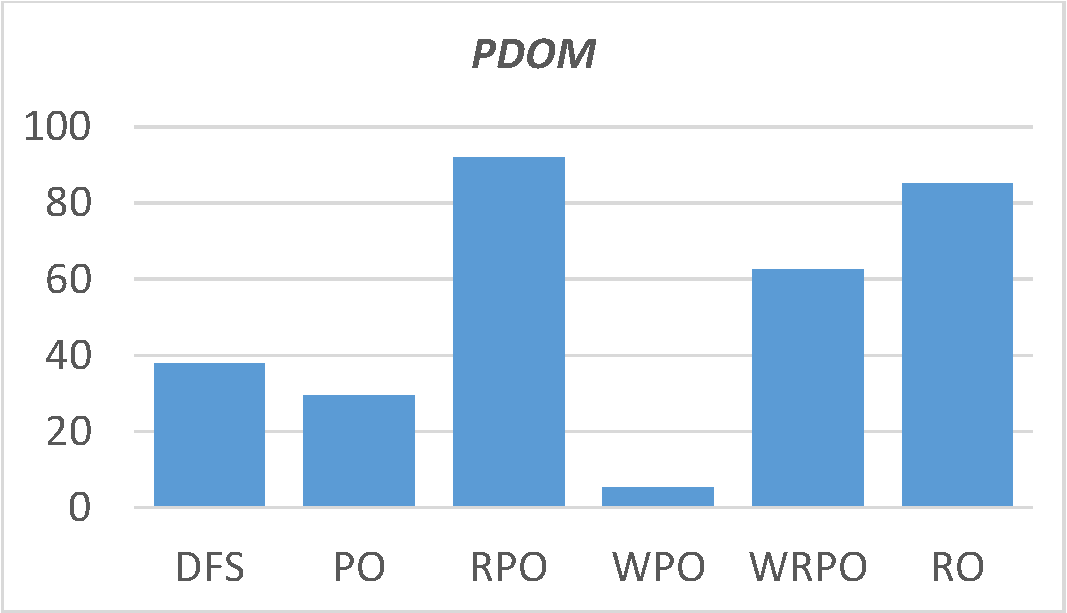
\includegraphics[width=0.32\linewidth]{ecoop-figures/pdom-crop.pdf}
%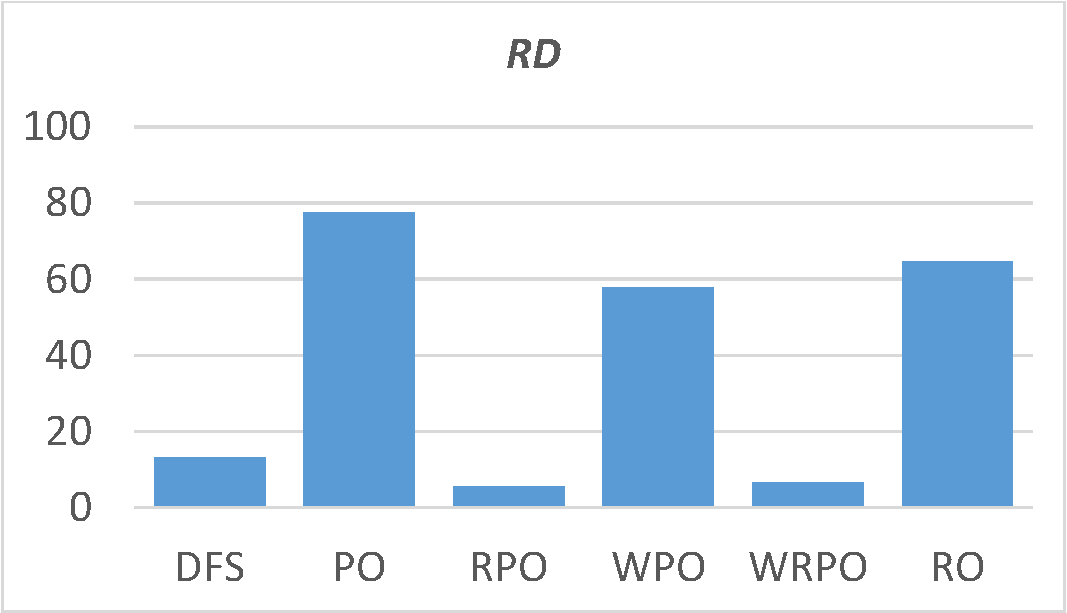
\includegraphics[width=0.32\linewidth]{ecoop-figures/rd-crop.pdf}
%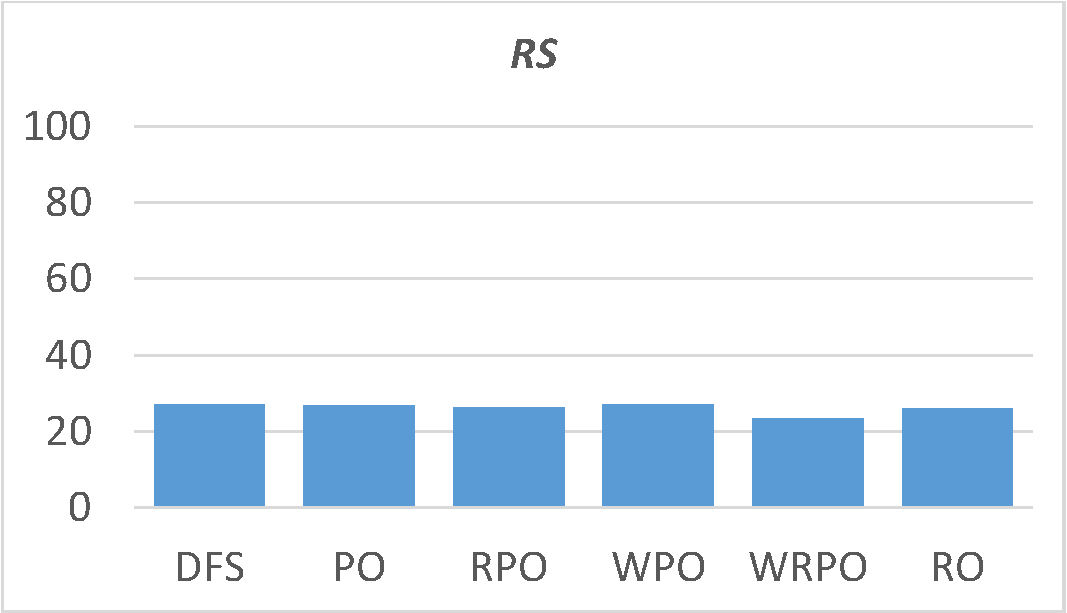
\includegraphics[width=0.32\linewidth]{ecoop-figures/rs-crop.pdf}
%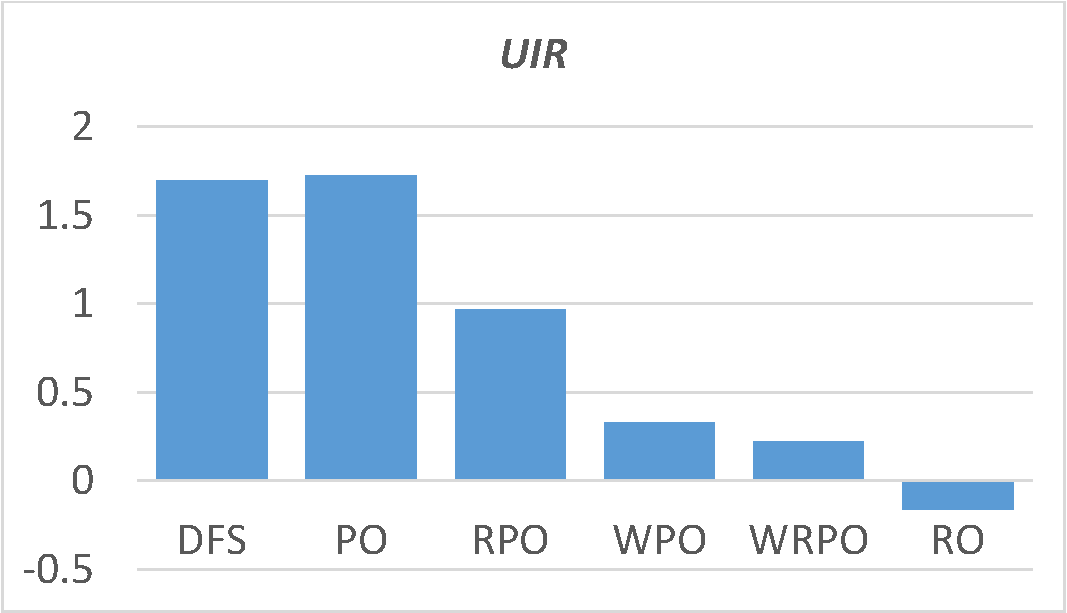
\includegraphics[width=0.32\linewidth]{ecoop-figures/uir-crop.pdf}
%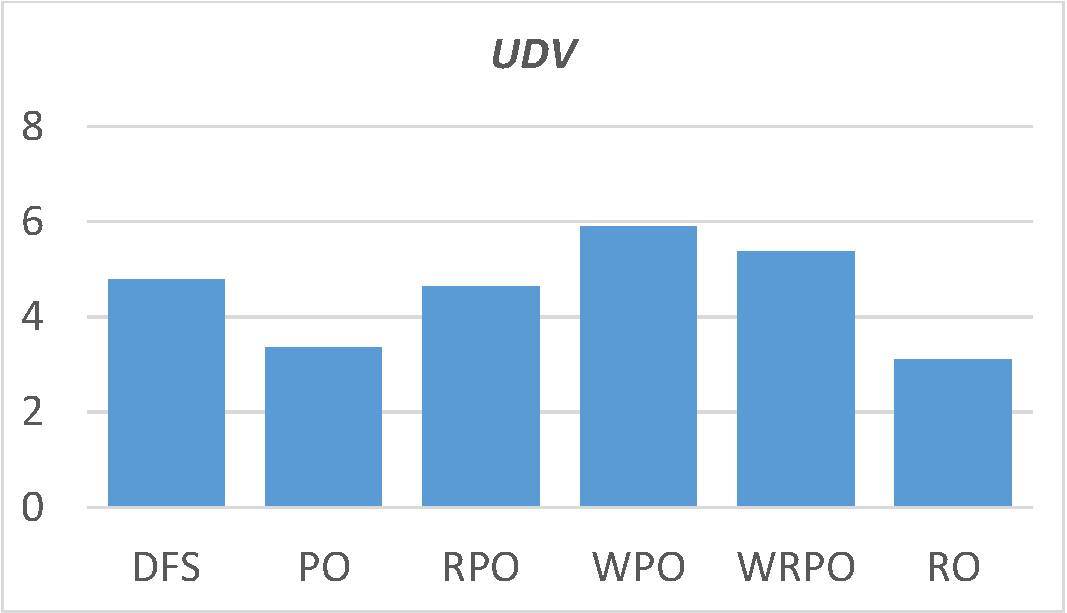
\includegraphics[width=0.32\linewidth]{ecoop-figures/udv-crop.pdf}
%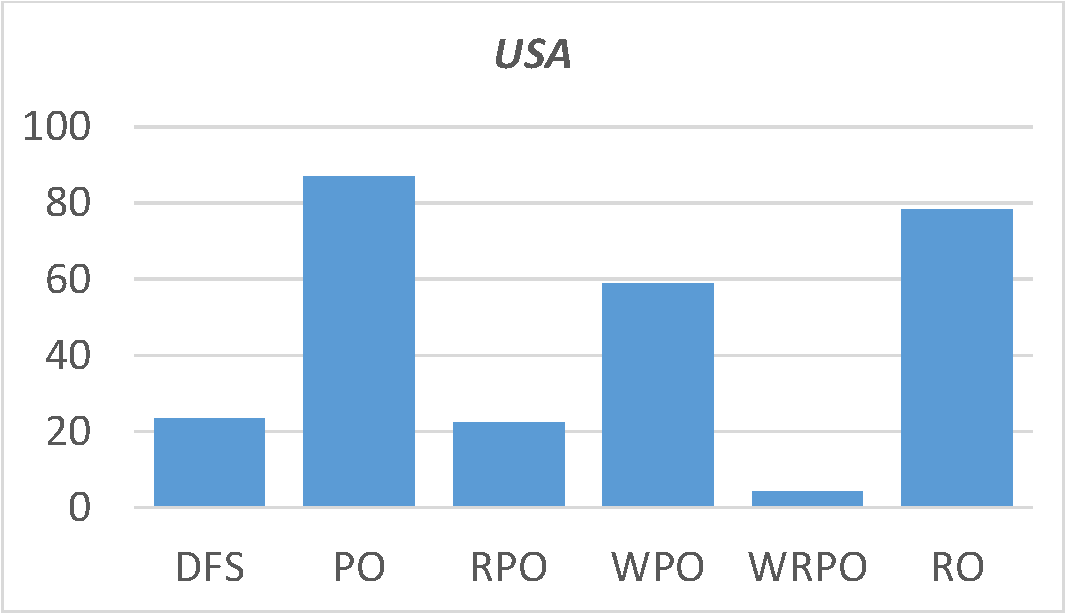
\includegraphics[width=0.32\linewidth]{ecoop-figures/usa-crop.pdf}
%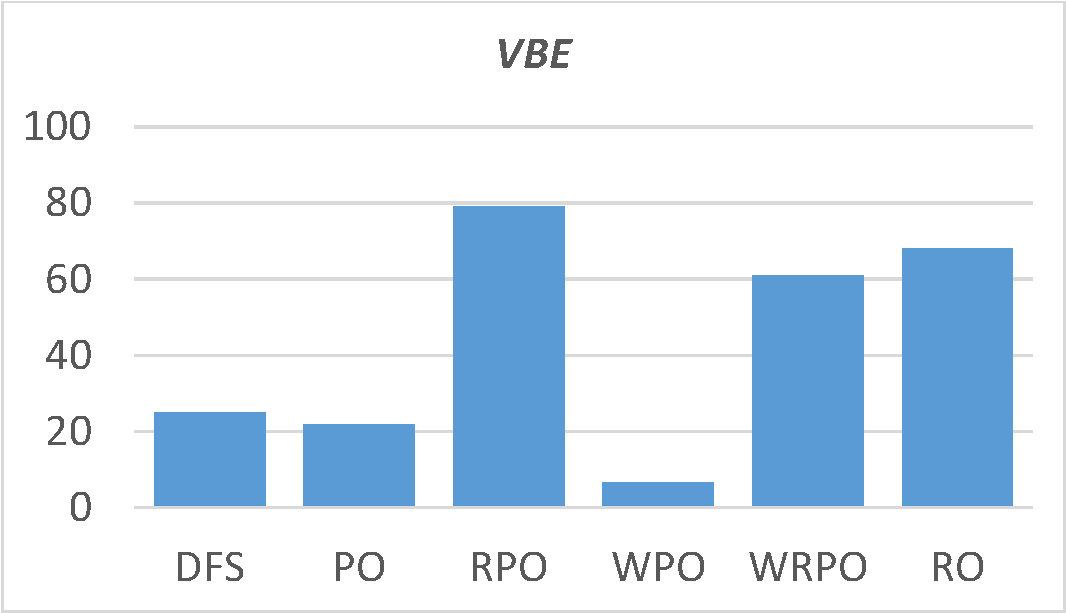
\includegraphics[width=0.32\linewidth]{ecoop-figures/vbe-crop.pdf}
%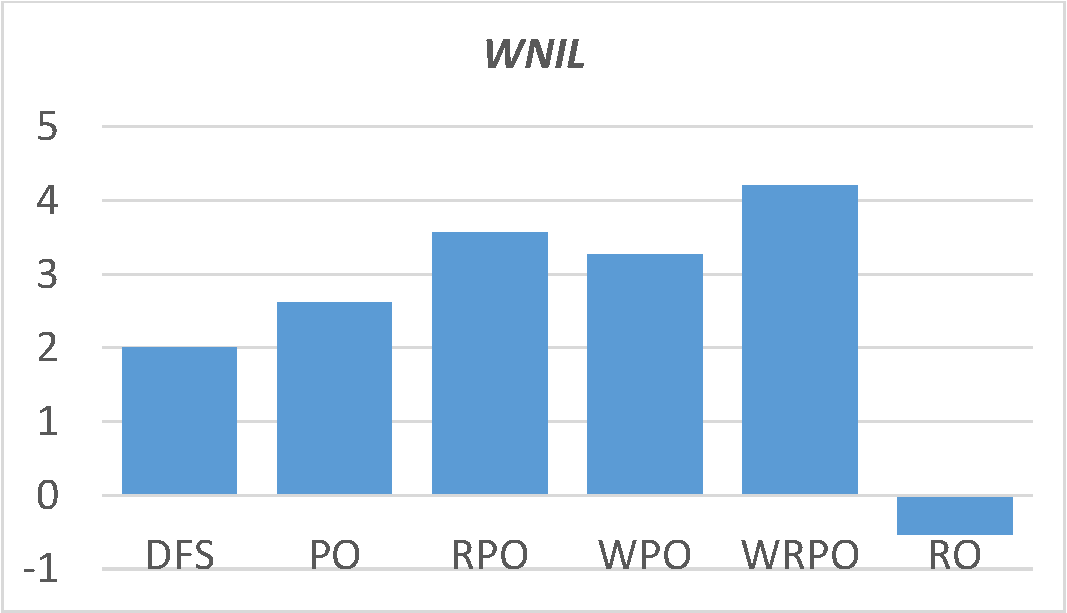
\includegraphics[width=0.32\linewidth]{ecoop-figures/wnil-crop.pdf}\newline
%\textbf{c) \textit{Overall}}\\
%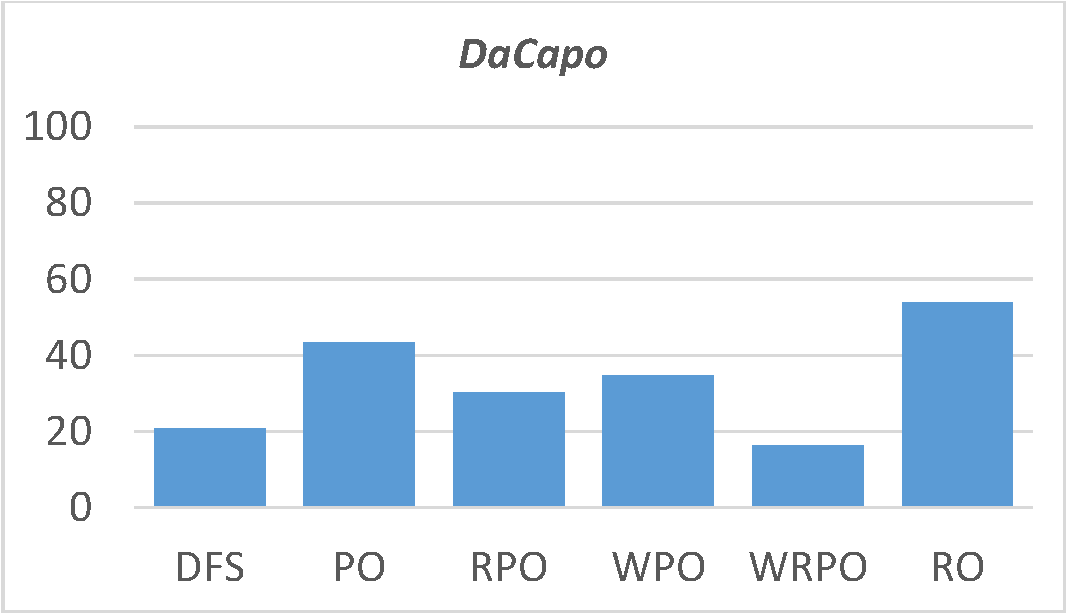
\includegraphics[width=0.32\linewidth]{ecoop-figures/dacapo-overall-crop.pdf}
  %\caption[Percentage reduction in execution time of hybrid approach over other candidate traversals on \textit{DaCapo} (Sequential mode) and \textit{SourceForge} (Cluster mode).]
%{Percentage reduction in execution time of hybrid approach over other candidate traversals on \textit{DaCapo} (Sequential mode) and \textit{SourceForge} (Cluster mode).
%\label{fig:dacapo-singlemachine-time-percentage}}
%\end{figure*}

%\begin{figure*}[ht!]
%\centering
%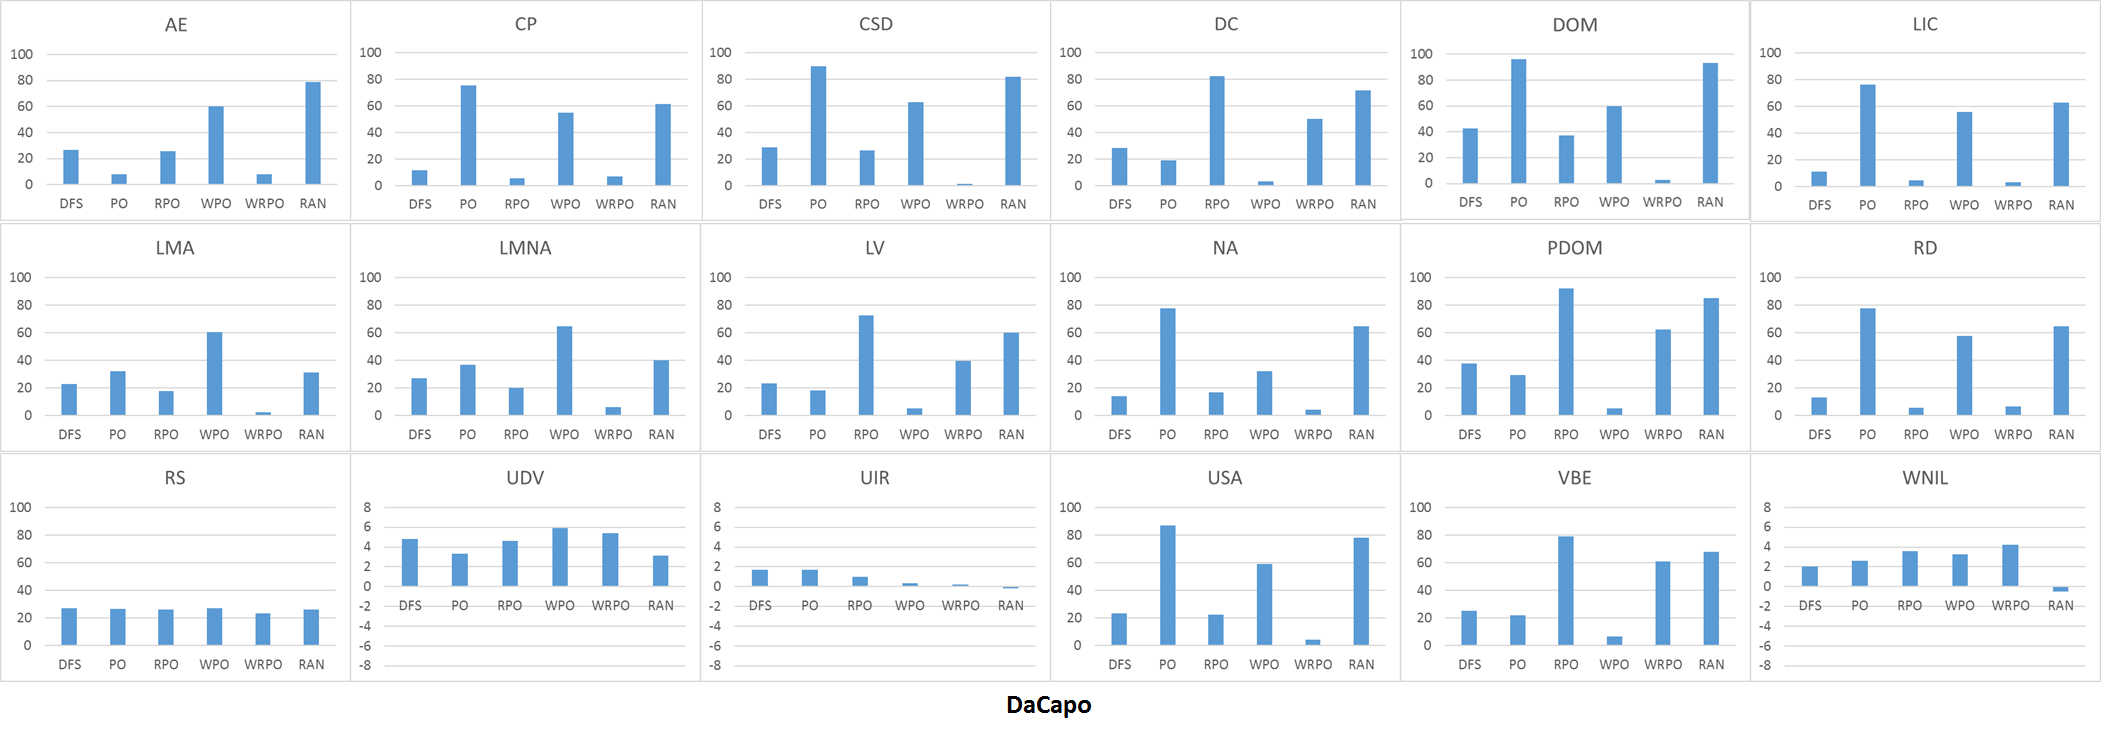
\includegraphics[width=\textwidth]{ecoop-figures/dacapo-seq-reduction.png}
%  \caption[Percentage reduction in execution time of hybrid approach over other candidate traversals on \textit{DaCapo} (Sequential mode), \textit{DaCapo} (Cluster mode), \textit{SourceForge} (Cluster mode).]
%{Percentage reduction in execution time of hybrid approach over other candidate traversals on \textit{DaCapo} (Sequential mode), \textit{DaCapo} (Cluster mode), \textit{SourceForge} (Cluster mode).
%\label{fig:dacapo-singlemachine-time-percentage}}
%\end{figure*}

\begin{figure*}[t]%
\centering
\scriptsize
\subfloat[Time reduction for each analysis.] {
\begin{tabular}{lrrrrrr|rrrrrr}
\toprule
\multicolumn{1}{l}{Analysis} & \multicolumn{6}{c|}{DaCapo}                    & \multicolumn{6}{c}{GitHub} \\
\cmidrule(lr){2-7} \cmidrule(lr){8-13}
      & DFS   & PO    & RPO   & WPO   & WRPO  & ANY    & DFS   & PO    & RPO   & WPO   & WRPO  & ANY \\
\midrule
\multicolumn{1}{l}{CP} & \cellcolor{lightblack}17\%  & \cellcolor{lightgreen}83\%  &  \cellcolor{lightblue}9\%   & \cellcolor{lightgreen}66\%  &  \cellcolor{lightblack}11\%   & \cellcolor{lightgreen}72\%  & \cellcolor{lightblack}17\%  & \cellcolor{lightgreen}88\%  &  \cellcolor{lightblack}12\%   & \cellcolor{lightgreen}80\%  &  \cellcolor{lightblue}5\%   & \cellcolor{lightgreen}82\% \\
\multicolumn{1}{l}{CSD} & \cellcolor{lightblack}41\%  & \cellcolor{lightgreen}93\%  & \cellcolor{lightblack}39\%  & \cellcolor{lightgreen}74\%  &  \cellcolor{lightblue}4\%   & \cellcolor{lightgreen}89\%  & \cellcolor{lightblack}31\%  & --  & \cellcolor{lightblack}24\%  & --  &  \cellcolor{lightblack}12\%   & -- \\
\multicolumn{1}{l}{DC} & \cellcolor{lightblack}41\%  & \cellcolor{lightblack}30\%  & \cellcolor{lightgreen}89\%  &  \cellcolor{lightblue}7\%   & \cellcolor{lightgreen}64\%  & \cellcolor{lightgreen}81\%  & \cellcolor{lightblack}25\%  & \cellcolor{lightblack}22\%  & --  &  \cellcolor{lightblue}7\%   & --  & -- \\
\multicolumn{1}{l}{LIC} & \cellcolor{lightblack}17\%  & \cellcolor{lightgreen}84\%  &  \cellcolor{lightblue}8\%   & \cellcolor{lightgreen}67\%  &  \cellcolor{lightblue}7\%   & \cellcolor{lightgreen}73\%  & \cellcolor{lightblack}19\%  & \cellcolor{lightgreen}89\%  &  \cellcolor{lightblack}15\%   & \cellcolor{lightgreen}81\%  &  \cellcolor{lightblack}19\%   & \cellcolor{lightgreen}88\% \\
\multicolumn{1}{l}{USA} & \cellcolor{lightblack}36\%  & \cellcolor{lightgreen}92\%  & \cellcolor{lightblack}34\%  & \cellcolor{lightgreen}72\%  &  \cellcolor{lightblue}9\%   & \cellcolor{lightgreen}87\%  & \cellcolor{lightblack}22\%  & --  & \cellcolor{lightblack}17\%  & --  &  \cellcolor{lightblue}9\%   & -- \\
\multicolumn{1}{l}{VFR} & \cellcolor{lightblack}20\%  & \cellcolor{lightblack}41\%  & \cellcolor{lightblack}18\%  & \cellcolor{lightgreen}51\%  & \cellcolor{lightblack}15\%  & \cellcolor{lightgreen}62\%  & \cellcolor{lightblack}15\%  & \cellcolor{lightblack}40\%  & \cellcolor{lightblue}10\%  & \cellcolor{lightblack}44\%  & \cellcolor{lightblue}9\%  & \cellcolor{lightgreen}53\% \\
\multicolumn{1}{l}{MWN} & \cellcolor{lightblack}21\%  & \cellcolor{lightblack}35\%  & \cellcolor{lightblack}16\%  & \cellcolor{lightblack}35\%  & \cellcolor{lightblack}22\%  & \cellcolor{lightblack}49\%  & \cellcolor{lightblack}17\%  & \cellcolor{lightblack}31\%  & \cellcolor{lightblack}12\%  & \cellcolor{lightblack}33\%  & \cellcolor{lightblack}11\%  & \cellcolor{lightblack}46\% \\
\multicolumn{1}{l}{AE} & \cellcolor{lightblack}40\%  &  \cellcolor{lightblack}14\%   & \cellcolor{lightblack}39\%  & \cellcolor{lightgreen}73\%  &  \cellcolor{lightblack}14\%   & \cellcolor{lightgreen}87\%  & \cellcolor{lightblack}16\%  &  --   & \cellcolor{lightblack}16\%  & --  &  \cellcolor{lightblack}11\%   & -- \\
\multicolumn{1}{l}{DOM} & \cellcolor{lightblack}54\%  & \cellcolor{lightgreen}97\%  & \cellcolor{lightblack}48\%  & \cellcolor{lightgreen}70\%  &  \cellcolor{lightblue}6\%   & \cellcolor{lightgreen}95\%  & \cellcolor{lightblack}27\%  & --  & \cellcolor{lightblack}32\%  & --  &  \cellcolor{lightblue}6\%   & -- \\
\multicolumn{1}{l}{LMA} & \cellcolor{lightblack}35\%  & \cellcolor{lightblack}46\%  & \cellcolor{lightblack}28\%  & \cellcolor{lightgreen}74\%  &  \cellcolor{lightblue}6\%   & \cellcolor{lightblack}46\%  & \cellcolor{lightblack}22\%  & --  & \cellcolor{lightblack}13\%  & --  &  \cellcolor{lightblue}6\%   & -- \\
\multicolumn{1}{l}{LMNA} & \cellcolor{lightblack}29\%  & \cellcolor{lightblack}39\%  & \cellcolor{lightblack}22\%  & \cellcolor{lightgreen}68\%  &  \cellcolor{lightblue}9\%   & \cellcolor{lightblack}41\%  & \cellcolor{lightblack}21\%  & --  & \cellcolor{lightblack}15\%  & --  &  \cellcolor{lightblue}7\%   & -- \\
\multicolumn{1}{l}{LV} & \cellcolor{lightblack}38\%  & \cellcolor{lightblack}30\%  & \cellcolor{lightgreen}84\%  &  \cellcolor{lightblack}11\%   & \cellcolor{lightblack}56\%  & \cellcolor{lightgreen}75\%  & \cellcolor{lightblack}25\%  & \cellcolor{lightblack}21\%  & \cellcolor{lightgreen}68\%  &  \cellcolor{lightblack}11\%   & \cellcolor{lightblack}69\%  & \cellcolor{lightgreen}80\% \\
\multicolumn{1}{l}{NA} & \cellcolor{lightblack}26\%  & \cellcolor{lightgreen}88\%  & \cellcolor{lightblack}30\%  & \cellcolor{lightblack}50\%  &  \cellcolor{lightblue}10\%   & \cellcolor{lightgreen}80\%  & \cellcolor{lightblack}13\%  & \cellcolor{lightgreen}87\%  & \cellcolor{lightblack}12\%  & \cellcolor{lightgreen}71\%  &  \cellcolor{lightblue}10\%   & \cellcolor{lightgreen}85\% \\
\multicolumn{1}{l}{PDOM} & \cellcolor{lightblack}51\%  & \cellcolor{lightblack}41\%  & \cellcolor{lightgreen}95\%  &  \cellcolor{lightblue}10\%   & \cellcolor{lightgreen}72\%  & \cellcolor{lightgreen}95\%  & \cellcolor{lightblack}24\%  & \cellcolor{lightblack}20\%  & --  &  \cellcolor{lightblack}24\%   & --  & -- \\
\multicolumn{1}{l}{RD} & \cellcolor{lightblack}15\%  & \cellcolor{lightgreen}80\%  &  \cellcolor{lightblue}7\%   & \cellcolor{lightgreen}62\%  &  \cellcolor{lightblue}9\%   & \cellcolor{lightgreen}68\%  & \cellcolor{lightblack}19\%  & \cellcolor{lightgreen}91\%  &  \cellcolor{lightblue}10\%   & \cellcolor{lightgreen}79\%  &  \cellcolor{lightblue}5\%   & \cellcolor{lightgreen}86\% \\
\multicolumn{1}{l}{RS} & \cellcolor{lightblack}31\%  & \cellcolor{lightblack}31\%  & \cellcolor{lightblack}30\%  & \cellcolor{lightblack}31\%  & \cellcolor{lightblack}28\%  & \cellcolor{lightblack}30\%  & \cellcolor{lightblack}16\%  & \cellcolor{lightblack}40\%  & \cellcolor{lightblue}9\%  & \cellcolor{lightblack}31\%  & \cellcolor{lightblue}7\%  & \cellcolor{lightblack}49\% \\
\multicolumn{1}{l}{VBE} & \cellcolor{lightblack}40\%  & \cellcolor{lightblack}36\%  & \cellcolor{lightgreen}88\%  &  \cellcolor{lightblack}13\%   & \cellcolor{lightgreen}76\%  & \cellcolor{lightgreen}81\%  & \cellcolor{lightblack}28\%  & \cellcolor{lightblack}24\%  & --  &  \cellcolor{lightblue}10\%   & --  & -- \\
\multicolumn{1}{l}{SS} & \cellcolor{lightblack}26\%  & \cellcolor{lightblack}39\%  & \cellcolor{lightblack}22\%  & \cellcolor{lightblack}37\%  & \cellcolor{lightblack}25\%  & \cellcolor{lightgreen}57\%  & \cellcolor{lightblack}20\%  & \cellcolor{lightblack}35\%  & \cellcolor{lightblack}13\%  & \cellcolor{lightblack}34\%  & \cellcolor{lightblue}10\%  & \cellcolor{lightgreen}50\% \\
\multicolumn{1}{l}{UDV} &  \cellcolor{lightblue}6\%   &  \cellcolor{lightblue}5\%   &  \cellcolor{lightblue}6\%   &  \cellcolor{lightblue}10\%   &  \cellcolor{lightblue}9\%   &  \cellcolor{lightblue}3\%   &  \cellcolor{lightblue}3\%   &  \cellcolor{lightblue}4\%   &  \cellcolor{lightblue}2\%   &  \cellcolor{lightblue}7\%   &  \cellcolor{lightblue}6\%   &  \cellcolor{lightblue}0\% \\
\multicolumn{1}{l}{UIR} &  \cellcolor{lightblue}2\%   &  \cellcolor{lightblue}2\%   &  \cellcolor{lightblue}1\%   & \cellcolor{lightblue}3\%   & \cellcolor{lightblue}3\%   & \cellcolor{lightblue}0\%   &  \cellcolor{lightblue}2\%   &  \cellcolor{lightblue}5\%   &  \cellcolor{lightblue}4\%   & \cellcolor{lightblue}7\%   & \cellcolor{lightblue}7\%   & \cellcolor{lightblue}0\% \\
\multicolumn{1}{l}{WNIL} &  \cellcolor{lightblue}3\%   &  \cellcolor{lightblue}4\%   &  \cellcolor{lightblue}5\%   &  \cellcolor{lightblue}6\%   &  \cellcolor{lightblue}8\%   & \cellcolor{lightblue}2\%  &  \cellcolor{lightblue}3\%   &  \cellcolor{lightblue}6\%   &  \cellcolor{lightblue}5\%   &  \cellcolor{lightblue}5\%   &  \cellcolor{lightblue}6\%   & \cellcolor{lightblue}0\% \\
\midrule
\multicolumn{1}{l}{Overall} &  \cellcolor{lightblack}31\%   &  \cellcolor{lightgreen}83\%   &  \cellcolor{lightgreen}70\%   &  \cellcolor{lightblack}55\%   &  \cellcolor{lightblack}35\%   &  \cellcolor{lightgreen}81\%   &  --   &  --  &  --   &  --   &  --  &  -- \\
\bottomrule
\end{tabular}%
\label{tab:reduction-analyses}
}\\
\subfloat[Overall reduction over analysis properties.] {
\setlength{\tabcolsep}{3.5pt}
\begin{tabular}{lrrrrrr}
\toprule
\multicolumn{1}{l}{Property} & \multicolumn{6}{c}{DaCapo}   \\
\cmidrule(lr){2-7}
      & DFS   & PO    & RPO   & WPO   & WRPO  & ANY   \\
\midrule
\multicolumn{1}{l}{Data-flow} & \cellcolor{lightblack}32\%  & \cellcolor{lightgreen}84\%  &  \cellcolor{lightgreen}72\%   & \cellcolor{lightgreen}57\%  &  \cellcolor{lightblack}36\%   & \cellcolor{lightgreen}83\% \\
\multicolumn{1}{l}{$\neg$Data-flow} & \cellcolor{lightblue}4\%  & \cellcolor{lightblue}4\%  & \cellcolor{lightblue}4\%  & \cellcolor{lightblue}6\%  &  \cellcolor{lightblue}6\%   & \cellcolor{lightblue}2\% \\
\bottomrule
\end{tabular}%
\label{tab:reduction-analysis-properties}
}
\subfloat[Overall reduction over graph properties.] {
\setlength{\tabcolsep}{3.5pt}
\begin{tabular}{lrrrrrr}
\toprule
\multicolumn{1}{l}{Property} & \multicolumn{6}{c}{DaCapo} \\
\cmidrule(lr){2-7} 
      & DFS   & PO    & RPO   & WPO   & WRPO  & ANY   \\
\midrule
\multicolumn{1}{l}{Sequential} & \cellcolor{lightblack}20\%  & \cellcolor{lightgreen}74\%  &  \cellcolor{lightgreen}63\%   & \cellcolor{lightgreen}55\%  &  \cellcolor{lightblack}28\%   & \cellcolor{lightgreen}72\%  \\
\multicolumn{1}{l}{Branch} & \cellcolor{lightblack}31\%  & \cellcolor{lightgreen}81\%  & \cellcolor{lightgreen}66\%  & \cellcolor{lightgreen}58\%  &  \cellcolor{lightblack}40\%   & \cellcolor{lightgreen}92\% \\
\multicolumn{1}{l}{Loop} & \cellcolor{lightgreen}53\%  & \cellcolor{lightgreen}88\%  & \cellcolor{lightgreen}75\%  &  \cellcolor{lightgreen}62\%   & \cellcolor{lightblack}37\%  & \cellcolor{lightgreen}95\% \\
\bottomrule
\end{tabular}%
\label{tab:reduction-graph-properties}
}
\caption{Reduction in running times.}
\label{fig:reduction}
\end{figure*}
